\chapter{Trabajo relacionado}\label{cap:conclusiones}
\noindent The present chapter describes other particular solutions for executing MapReduce applications. Each one's characteristics will be briefly explored by contrasting them against qosh's.

\section{Amazon Elastic MapReduce}\label{sec:emc}
\noindent \emph{Amazon Elastic MapReduce} \cite{aws} exposes a web service interface that allows the user to send MapReduce execution requests. EMR is supported internally by Amazon EC2 to provision, on demand, the required infrastructure by the MapReduce work flow. Thus, an EMR user will not have to worry about provisioning, creating, configuring and destroying the virtual clusters that would support execution. This convenient transparency to the user comes with a series of important limitations:

\begin{description}
    \item[Underlying infrastructure restriction]: being as it is a service owned by Amazon, it was expected that usage of computational resources out of their reach were limited; and so it is: EMR users will not be able to couple their virtual instances to other clouds that may incur in lower exploitation costs.
    qosh, as it has been shown, separates and exposes responsibilities in a way that using a different cloud, for example, requires only adapting a new Compute module to the particular REST API of the cloud that would be used.
    \item[Installation restriction]: it is not possible to deploy a custom-built VM to execute MapReduce applications in EMR. qosh will handle work flows driving a Hadoop VM with a loose coupling with the deploying subsystem (Fabric) with a doble end:
    \begin{itemize}
        \item To ease VM customizations and upgrades (Kernel, Hadoop, JRE, etc.).
        \item To give the possibility to create custom VMs from scratch.
    \end{itemize}
    \item[Information restriction:] some users are under non disclosure agreements that render impossible sharing data with third parties like Amazon, effectively leaving those services out of the equation. qosh's open source nature makes it easy for a developer to adapt qosh to its concrete functional requirements with no sharing of private data.
\end{description}

EMR node typology is described next. EMR clusters present three kinds of nodes:

\begin{description}
    \item[Master:] this node, unique per EMR cluster, executes both a NameNode and a JobTracker.
    \item[Core:] this kind of nodes store data and process job tasks. The are basically comprised of a DataNode and a TaskTracker.
    \item[Task:] they only run TaskTracker processes.
\end{description}

qosh deploys clusters with a single hybrid master-worker node --- with NameNode, JobTracker, DataNode and TaskTracker --- being the rest worker nodes --- with DataNode and TaskTracker only. This deployment configuration could be easily altered to fit into diverse use cases by rewriting the \texttt{mapred.fabric.fabfile} module.

Regarding the execution flow, EMR allows for keeping the instances alive when they had finished scheduled processing to avoid the computational overhead of their spawning. qosh's default behavior is to destroy instances upon completion. As expected, defaults may be easily overridden.

EMR draws on Amazon S3 to store input data to Hadoop as well as to write final results. Intermediate information is stored within the virtual instances and is destroyed as they are. qosh uses the file system of the Controller Node to store I/O data from the virtual cluster, and, like EMR, employs the virtual instances' file system to save intermediate data. qosh may also be plugged a different repository to store final results. To that end, a new back end module would have to be written for Django to correctly locate data and update the DB to point elsewhere.

\section{Resilin}\label{sec:resilin}
\noindent \emph{Resilin} \cite{resilin} main intention is to improve EMR by trying to overcome its limitations. The development team has written an API (see figure \ref{fig:arquitecturaresilin}) capable of receiving EMR-like requests that will translate into two kinds of actions:

\begin{itemize}
    \item An interaction flow with an IaaS Cloud to create and destroy instances (what qosh does in its Compute module).
    \item An SSH connection to the virtual Hadoop cluster to configure and execute tasks (what qosh does with its Fabric module).
\end{itemize}

\begin{figure}[tbp]
\begin{center}
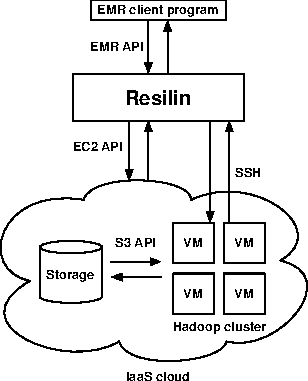
\includegraphics[width=0.5\textwidth]{imagenes/035.pdf}
 \caption{Resilin architecture. Source: \cite{resilin}}
\label{fig:arquitecturaresilin}
\end{center}
\end{figure}

Information storage and I/O is delegated upon an S3 compatibility adaptor supported both by Nimbus and Eucalyptus --- with \emph{Cumulus} and \emph{Walrus} respectively.

Besides, and maybe the most interesting Resilin trait, its implementors experiment with the possibility to execute MapRecude work flows atop infrastructure provided by different clouds. Though it may not be the general approach to provision private infrastructure to virtual deployments due to the inherent heterogeneity among different IaaS frameworks, it might prove useful when the infrastructure has to be drawn upon from public clouds. In the abstract, the idea has been implemented bridging deployments on different clouds by exposing instances on one cloud to the other cloud Master Node as if they were part of the same virtual cluster.

qosh does not support hybrid cloud deployments. Yet, it cloud be implemented without much ado modifying the Compute module accordingly.

The bottom line is that Resilin is the solution resembling qosh the most; delegating the reduction of MapReduce work flows on Hadoop and the virtual deployments on an IaaS Cloud EC2-compatible --- all of the four evaluated in \ref{sec:frameworksevaluados} are. Lastly, figure \ref{fig:resilinproyecto} lists the different tools that aid supporting the functionality exposed.

\begin{figure}[tbp]
\begin{center}
\begin{tabular}{|c|c|c|}
\hline
& \textbf{Resilin} & \textbf{qosh} \\
\hline
\textbf{Global} & \texttt{Python} & \texttt{Python} \\
\hline
\textbf{HTTP} & \texttt{Twisted} & \texttt{Django} \\
\hline
\textbf{IaaS Cloud interaction} & \texttt{boto} & \texttt{Compute} (custom module) \\
\hline
\textbf{Virtual instances interaction} & \texttt{paramiko} & \texttt{Fabric} \\
\hline
\end{tabular}
\caption{Tool listing}
\label{fig:resilinproyecto}
\end{center}
\end{figure}

\section{Cloud MapReduce}\label{sec:cloudmapred}
\noindent \emph{Cloud MapReduce} representa una aproximaci\'on diametralmente opuesta a Resilin. Mientras Resilin pretende implementar un API MapReduce centr\'andose en \emph{organizar} los distintos componentes necesarios, Cloud MapReduce se apoya en los servicios de un cloud ---en concreto el de Amazon--- para implementar el modelo MapReduce \cite{googlemapreduce} \emph{directamente} sobre \'el.\newline

A continuaci\'on comentamos algunas propiedades de Cloud MapReduce que consideramos m\'as relevantes:

\begin{description}
\item[Escalabilidad incremental:] es la capacidad de a\~nadir nuevos nodos al cl\'uster MapReduce cuando el trabajo ya ha comenzado; de tal forma que las nuevas instancias se informen autom\'aticamente del estado global del trabajo y se asignen tareas ellas mismas. Resilin \cite{resilin} lo soporta tambi\'en, nuestro proyecto no.
\item[Simetr\'ia y descentralizaci\'on:] con esta idea se pone manifiesto la falta de jerarqu\'ia en los despligues: cada nodo de un cl\'uster tendr\'a las mismas responsabilidades que sus colegas. Este representa el primer punto de distinci\'on importante frente a las dem\'as aproximaciones ---MapReduce, Hadoop, Amazon EMR, Resilin y nuestro proyecto--- en las que la configuraci\'on, reparto, planificaci\'on, etc. de los trabajos y tareas tiene lugar dentro de los nodos maestro, y la ejecuci\'on y almacenamiento sucede en los esclavos. En Cloud MapReduce los nodos act\'uan de modo independiente, controlando el estado global del trabajo para determinar qu\'e tarea se adec\'ua mejor a las necesidades instant\'aneas del flujo de trabajo. Se debe citar asimismo, que esta simetr\'ia de Cloud MapReduce hace que sea menos problem\'atico superar los problemas en los maestros.
\item[Heterogeneidad:] entendida con una doble componente: por una parte, la posible coexistencia de instancias de distintos \emph{sabores} ---siguiendo la notaci\'on de Amazon--- en un mismo trabajo, y por la otra, la capacidad de crear instancias en m\'ultiples clouds. Resilin soporta ambas cuestiones, nuestra propuesta no.
\end{description}

En Cloud MapReduce el almacenamiento global ---la E/S y los datos intermedios--- se hace sobre S3, la comunicaci\'on y sincronizaci\'on entre nodos con el servicio de colas de Amazon (\emph{SQS} o \emph{Simple Queue Service}) y el almacenamiento de estado de las tareas y nodos en el servicio de base de datos de Amazon, \emph{SimpleDB}. En nuestro proyecto, el almacenamiento global se hace sobre el sistema de ficheros del servidor web; que probablemente no sea la mejor opci\'on debido a las limitaciones de ancho de banda y la falta de tolerancia a fallo. Para modificar este comportamiento, ser\'ia necesario, por ejemplo, dise\~nar un backend de datos personalizado y acoplarlo al \emph{pipe} de almacenamiento de Django, o montar alg\'un sistema de ficheros y apuntar a Django en su direcci\'on. En cuanto a la sincronizaci\'on, comunicaci\'on y estado de las instancias, se delega toda esa funcionalidad en Hadoop.\newline

Por \'ultimo se presenta la figura \ref{fig:arquitecturacloudmapreduce}, que recoge la instant\'anea de alto nivel de un instante de la ejecuci\'on de un trabajo en el Cloud MapReduce. Esta figura recuerda, y no casualmente, a la figura \ref{fig:exmapreduce} que presentaba las fases t\'ipicas de procesamiento del paradigma MapReduce original \cite{googlemapreduce}.

\begin{figure}[tbp]
\begin{center}
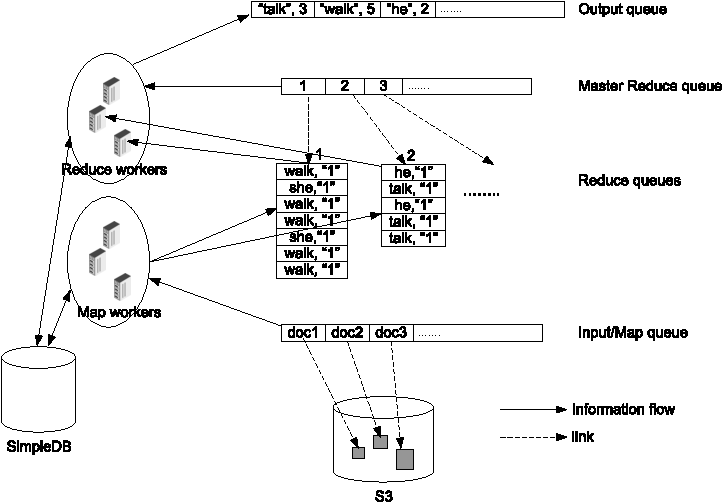
\includegraphics[width=0.9\textwidth]{imagenes/036.pdf}
 \caption{Arquitectura de Cloud MapReduce. Fuente: \cite{cloudmapreduce}}
\label{fig:arquitecturacloudmapreduce}
\end{center}
\end{figure}

\section{Dynamic Cloud MapReduce}\label{sec:dynamicmapreduce}
\hyphenation{SmartFrog}
\noindent La figura \ref{fig:arquitecturadynamicmapreduce} presenta la arquitectura de la soluci\'on propuesta en \cite{dynamicmapreduce} para la apropiaci\'on y configuraci\'on autom\'aticas de infraestructura virtual que procesar\'a aplicaciones MapReduce. Como se ve, los componentes de alto nivel se corresponden directamente con los de nuestra aproximaci\'on; sin embargo (\emph{Dynamic Cloud MapReduce}) presenta algunas diferencias.

\begin{figure}[tbp]
\begin{center}
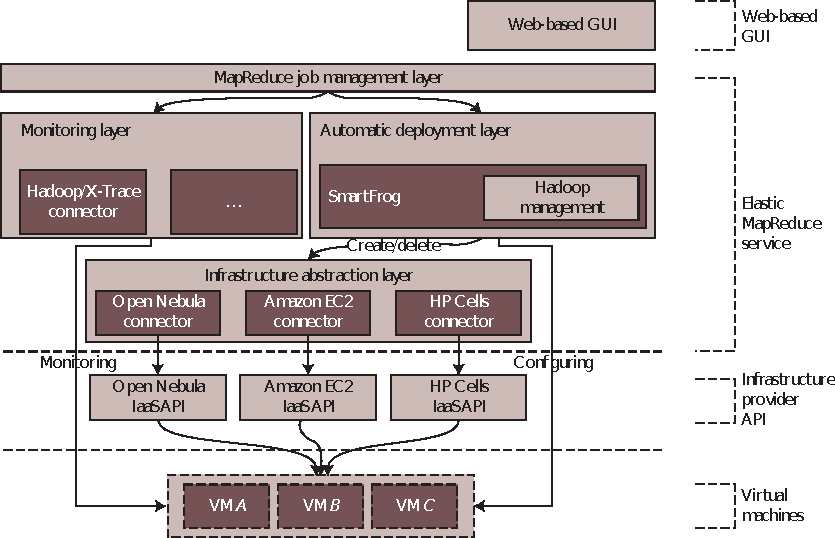
\includegraphics[width=0.9\textwidth]{imagenes/037.pdf}
 \caption{Dynamic Cloud MapReduce. Fuente: \cite{dynamicmapreduce}}
\label{fig:arquitecturadynamicmapreduce}
\end{center}
\end{figure}

\begin{description}
\item[GUI:] a pesar de que la interfaz con el usuario tambi\'en es una p\'agina web, en este caso han implementado un servicio \emph{RESTful} (la capa de direcci\'on de los trabajos MapReduce) que desacopla el manejo del servicio de procesamiento MapReduce. Adem\'as, dicha capa permite que los usuarios del despliegue encadenen la ejecuci\'on de m\'ultiples trabajos MapReduce. En nuestra propuesta hemos implementado las acciones de despliegue y procesado formando parte de la mec\'anica de la web. Este \'ultimo punto, el encadenamiento de flujos MapReduce, no se soporta.
\item[Monitoring Layer:] como su nombre indica, es una capa orientada a la monitorizaci\'on de los procesos MapReduce. Si bien no hemos integrado esta caracter\'istica en la interfaz web, tampoco hemos limitado el acceso a los servicios de monitorizaci\'on integrados en Hadoop; en referencia a los comentados microservidores web de cada m\'odulo \emph{Tracker}.
\item[Automatic Deployment Layer:] con esta capa software se controla el des\-plie\-gue virtual. Equivale a nuestro m\'odulo \emph{Fabric} (\texttt{fabfile.py}). La diferencia fundamental, a parte de que usan \emph{SmartFrog} para gestionar el despliegue, es que la m\'aquina virtual parte de una instalaci\'on \emph{limpia} del sistema operativo a la que se le ha agregado exclusivamente  SmartFrog. De manera que, antes de ejecutar cada flujo MapReduce, SmartFrog gestiona la descarga, instalaci\'on y configuraci\'on de Hadoop en cada m\'aquina virtual. Esta aproximaci\'on es m\'as flexible que la propuesta en el proyecto ---nos apoyamos en una imagen con Hadoop y el JRE preinstalados---, pero a\~nade una importante sobrecarga de descarga y configuraci\'on.
\item[Infrastructure Provider Abstraction Layer:] con esta fachada separan la sintaxis del servicio REST del cloud concreto desplegado, permitiendo definir adaptadores para cada uno. En nuestra propuesta no hemos aislado una interfaz que permita definir adaptadores de forma transparente. Sin embargo, y tal como se ha apuntado, bastar\'ia definir el comportamiento de las funciones del m\'odulo \texttt{Compute} (\texttt{compute.py}) y adaptar los \emph{Transfer Objects} (\texttt{objects.py}) a cada sintaxis.
\end{description}

Por \'ultimo, hacer constar que la opci\'on elegida para el almacenamiento es muy parecida a la propuesta ---\emph{HDFS} y sistema de ficheros local. Sin embargo, nuestra soluci\'on es autom\'atica: no requiere que el usuario suba manualmente los ficheros de entrada. Los ficheros de salida se almacenan en un servidor local y son accesibles desde la interfaz REST. En nuestra propuesta se permite que cada usuario descargue los resultados de sus procesamientos desde la interfaz web.

\section{Resumen}\label{sec:resumenconclusiones}
\noindent Teniendo en cuenta lo expuesto hasta este punto, se podr\'ia pensar que nuestra implementaci\'on es la m\'as limitada. Sin embargo, presenta una importante ventaja frente a todas las dem\'as solucciones: la \emph{absoluta simplicidad}. Lo que parece un car\'acter secundario se convierte en algo fundamental si el usuario es inexperto o si se pretende hacer un despliegue r\'apido de tecnolog\'ia MapReduce el\'astica.\newline

Ninguna de las soluciones estudiadas presenta una aproximaci\'on tan simple e integrada de instalaci\'on, configuraci\'on y explotaci\'on de infraestructura. Todas conllevan alg\'un esfuerzo adicional del usuario, requiriendo, en general: el conocimiento de su mec\'anica interna, el despliegue previo de un cloud, el abono bajo consumo o el hacer p\'ublicos los datos de entrada al framework MapReduce. En resumen, nuestro proyecto es la elecci\'on natural para des\-plie\-gues reducidos inicialmente o como punto introductorio a las tecnolog\'ias cloud IaaS y MapReduce. Partiendo de un despligue m\'inimo y autom\'atico, el administrador del cloud podr\'a agregar nuevos nodos de procesamiento, ac\-tua\-li\-zar la m\'aquina virtual Hadoop, alterar la mec\'anica de aprovisionamiento o, incluso, instalar un cloud de otro proveedor, sin demasiado esfuerzo.
